\chapter{Model Fitting and Optimization}
\section{Optimization(优化)}
\begin{align*}
    \text{minimize }& f_0(x)\\
    \text{subject to }&f_i(x)\le 0 ,i=1,\cdots ,m\\
    &g_i(x)=0, i=1,\cdots ,p
\end{align*}
\begin{enumerate}
    \item $x\in R^n$(vector) is \transtip{优化变量}{variable} to be chosen. 
    \item $f_0(x)$ is the \transtip{目标函数}{objective function} to be minimized.
    \item $f_1,\cdots,f_m$ are the \transtip{不等式约束条件}{inequality constraint functions}.
    \item $g_1,\cdots,g_m$ are the \transtip{等式约束条件}{equality constraint functions}.
\end{enumerate}

eg: Image deblurring.
\begin{align*}
    \min_{X}& \left\| Y-F*X \right\|_{2}^{2} \text{(用范数衡量向量大小)}\\
    Y: &\text{Blurred image}\\
    F: &\text{Blur kernel}\\
    X: &\text{Sharp image}
\end{align*}

\section{Model fitting}
\subsection{Model}
A model describes the relationship between input and output(输入与输出的关系).

eg: linear model
\begin{align*}
    b&=a^Tx\\
    a& \text{ is input}\\
    b& \text{ is output}\\
    x& \text{ is model parameter(参数)}
\end{align*}
\begin{figure}[H]
    \centering
    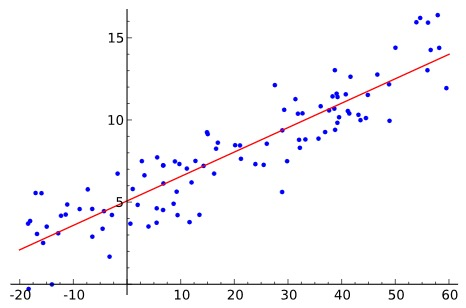
\includegraphics[width=0.38\textwidth]{Lec4/linear model}
\end{figure}
\subsection{Model fitting(Learning)}
To estimate model parameters from data.

A typical approach: Minimize the \transtip{最小均方误差}{Mean Square Error}(MSE).
\begin{align*}
    \hat{x}=\arg \min_x\sum_i(b_i-a_i^Tx)^2
\end{align*}

Why use MSE?
\subsection{Maximum Likelihood Estimate(MLE,极大似然估计)}
参数能最大化这组数据出现的概率.(目标函数是用噪声分布推导而出的)
\begin{enumerate}
    \item 假设数据噪声是Gaussian分布.(最常用的是Gaussian, 因为各种随机变量的和可以证明是一个Gaussian? 所以在噪声未先验的情况下Gaussian最保险)
    \begin{align*}
        b_i=a_i^Tx+n, n\sim G(0,\sigma)
    \end{align*}
    \item 给定x, 观测到$(a_i,b_i)$的可能性为:
    \begin{align*}
        P[(a_i,b_i)|x]=P[b_i-a_i^Tx]\varpropto \exp(-\frac{(b_i-a_i^Tx)^2}{2\sigma^2})
    \end{align*}
    
    $P$就是likelihood(可能性,不是概率)

    \item 给很多点
    \begin{align*}
        &P[(a_1,b_1)\dots|x]\\
        =&\prod_i P[(a_i,b_i)|x]\\
        =&\prod_i P[b_i-a_i^Tx]\\
        \varpropto& \exp(-\frac{(b_i-a_i^Tx)^2}{2\sigma^2})=\exp(-\frac{\left\| Ax-b \right\|_2^2}{2\sigma^2})
    \end{align*}

    \item MLE=寻找最大化$P[(a_1,b_1)\dots|x]$的$x$, 即
    \begin{align*}
        \hat{x}&=\arg \max_x P[(a_1,b_1)\dots|x]\\
        &=\arg \max_x \exp(-\frac{\left\| Ax-b \right\|_2^2}{2\sigma^2})\\
        &=\arg \min_x \left\| Ax-b \right\|_2^2
    \end{align*}
    \item MSE=MLE with Gaussian noise assumption(高斯假设下的MLE)
\end{enumerate}

\section{Numerical methods}

\subsection{Problems have analytical solution}
    对有解析解的问题

    eg:Linear MSE

    求导, 让导数等于0. 但矩阵求导比较复杂, 需要网上去搜().
    \begin{align*}
        \hat{x}&=\arg \min_x \left\| Ax-b \right\|_2^2\\
    \end{align*}

    对上式求导:
    \begin{align*}
        \hat{x}'=A^T(Ax-b)\\
    \end{align*}

    令其为0,有:
    \begin{align*}
        A^TAx=A^Tb
    \end{align*}

    求解即得$\hat{x}$

\subsection{No analytical solution}
    使用数值方法: 梯度下降(Gradient descent).

    \begin{align*}
        F(x_0)>F(x_1)>\dots >F(x_k)>\dots
    \end{align*}
    \begin{figure}[H]
        \centering
        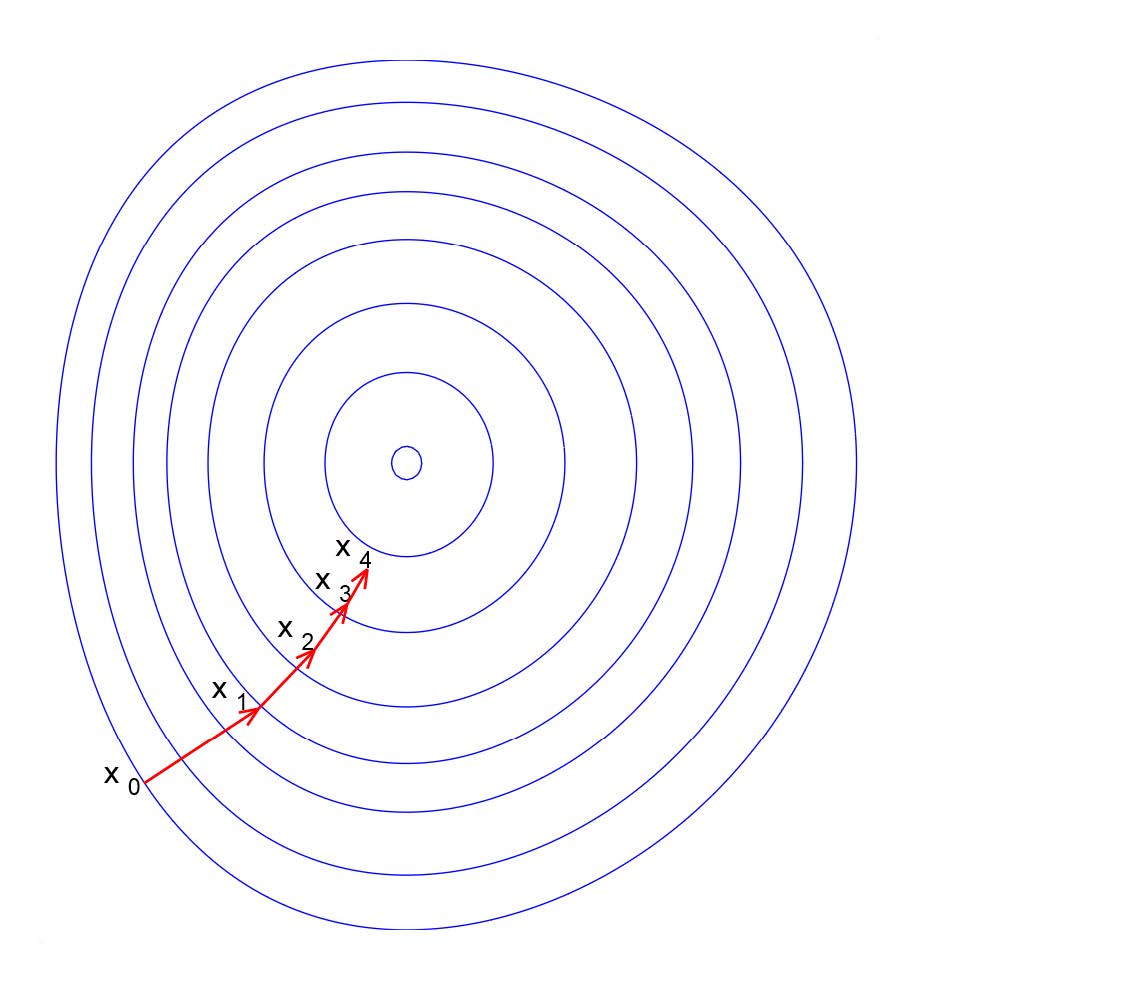
\includegraphics[width=0.22\textwidth]{Lec4/梯度下降}
        \caption{Gradient descent}
    \end{figure}
    \begin{algorithm}[H]
        \caption{Gradient descent}
        \begin{algorithmic}[1]
            \State $x$ \gets $x_0$ \Comment{Init}
            \While{not converge}
                \State h \gets descending\_direction$(x)$ \Comment{determine the direction}
                \State $\alpha$ \gets descending\_step$(x,h)$ \Comment{determine the step}
                \State x \gets $x+\alpha h$ \Comment{update the parameters}
            \EndWhile
        \end{algorithmic}
    \end{algorithm}
    So how to find $h$ and $\alpha$
    \subsubsection{Taylor expansion}
    \begin{enumerate}
        \item First-order approximation
        \begin{align*}
            F(x_k+\Delta x) &\approx F(x_k)+J_F\Delta x\\
            \mathbf{J}&=\begin{bmatrix}
                \frac{\partial f}{\partial x_1} &\cdots &\frac{\partial f}{\partial x_n}
            \end{bmatrix}
        \end{align*}
        $J_F$ is Jacobian matrix, also as first-order derivative.
        \item Second-order approximation
        \begin{align*}
            F(x_k+\Delta x) &\approx F(x_k)+J_F\Delta x+\frac{1}{2}\Delta x^T H_F \Delta x\\
            \mathbf{H}&=\begin{bmatrix}
                \frac{\partial^{2} f}{\partial x_{1}^{2}} & \frac{\partial^{2} f}{\partial x_{1} \partial x_{2}} & \cdots & \frac{\partial^{2} f}{\partial x_{1} \partial x_{n}} \\
                \frac{\partial^{2} f}{\partial x_{2} \partial x_{1}} & \frac{\partial^{2} f}{\partial x_{2}^{2}} & \cdots & \frac{\partial^{2} f}{\partial x_{2} \partial x_{n}} \\
                \vdots & \vdots & \ddots & \vdots \\
                \frac{\partial^{2} f}{\partial x_{n} \partial x_{1}} & \frac{\partial^{2} f}{\partial x_{n} \partial x_{2}} & \cdots & \frac{\partial^{2} f}{\partial x_{n}^{2}}
                \end{bmatrix}
        \end{align*}
        $H_F$ is Hessian matrix, also as second-order derivative.
    \end{enumerate}

    \subsubsection{Gradient descent(GD)}
        
    假设目标函数近似为:
    \begin{align*}
        F(x_k+\Delta x) &\approx F(x_k)+J_F\Delta x
    \end{align*}

    当$J_F\Delta x<0$时, 目标函数会变小.
    
    Steepest descent method(最速梯度下降法)
    
    当$\Delta x$与$J_F$(一阶近似)方向完全一致, 即$\Delta x=-J_F^T$时, 下降最快.  

    Determine the step size:
    \begin{enumerate}
        \item Exact line search(一个个去试)
        \item Backtracking algorithm(回溯法)(求一个可接受的解)
        \begin{itemize}
            \item Initialize $\alpha$ with a big value.
            \item Decrease $\alpha$ until $\Phi(\alpha)\le\Phi(0)+\gamma\Phi'(0)\alpha$
            
            $\gamma$ is a parameter, $0<\gamma<1$
        \end{itemize}
        \begin{figure}[H]
            \centering
            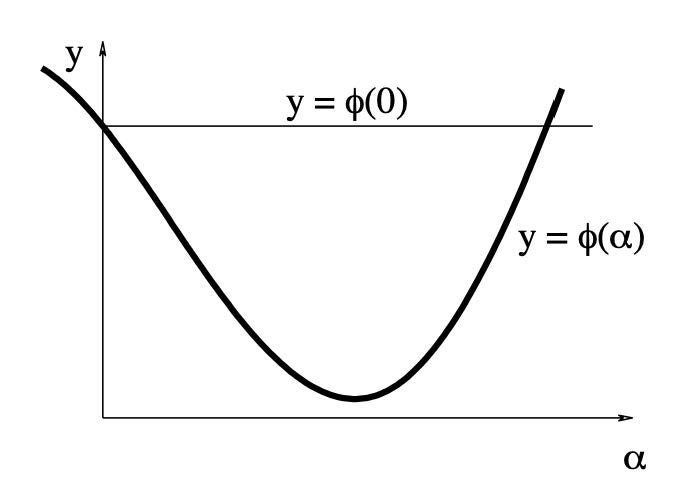
\includegraphics[width=0.22\textwidth]{Lec4/Exact line search}
            \caption{$\Phi(\alpha)=F(\mathrm{x}+\alpha \mathrm{h})$, $\mathrm{x}$ and $\mathrm{h}$ fixed, $\alpha\ge0$}
        \end{figure}
    \end{enumerate}
    \begin{itemize}
        \item Advantage: 简单, 较远时效果好.
        \item Disadvantge: 越接近收敛越慢, 计算浪费多.
    \end{itemize}

    \subsubsection{Newton method }
    \begin{align*}
        F(x_k+\Delta x) &\approx F(x_k)+J_F\Delta x+\frac{1}{2}\Delta x^T H_F \Delta x
    \end{align*}

    Find $\Delta x$ to minimize $F(x_k+\Delta x)$,(求导)
    \begin{align*}
        H_F\Delta x+J_F^T=0
    \end{align*}

    The optimal direction(Newton step),
    \begin{align*}
        \Delta x=-H_F^{-1}J_F^T
    \end{align*}
    \begin{itemize}
        \item Advantage: 在最小点附近收敛更快
        \item Disadvantge: Hessian需要更大计算量, 甚至无法计算
    \end{itemize}

    \subsubsection{Gauss-Newton method(仅求解非线性最小二乘)}
    \begin{align*}
        \hat{x}&=\arg\min_xF(x)\\
        &=\arg\min_x\left\| R(x) \right\|_2^2\\
        R(x)&=\begin{bmatrix}
            b_1-f_x(a_1)\\
            b_2-f_x(a_2)\\
            \vdots\\
            b_n-f_x(a_n)
        \end{bmatrix}
    \end{align*}

    $R(x)$ is residual vector(残差向量)

    展开$R(x)$,
    \begin{align*}
        \left\| R(x_k+\Delta x) \right\|_2^2 &\approx \left\| R(x_k)+J_R\Delta x \right\|_2^2\\
        &=\left\| R(x_k) \right\|_2^2+2R(x_k)^TJ_R\Delta x+\Delta x^T J_R^T J_R \Delta x
    \end{align*}

    The optimal $\Delta x$ satisfies,(求导)
    \begin{align*}
        J_R^T J_R \Delta x+J_R^T R(x_k)=0
    \end{align*}

    $J_R$ is the Jacobian of $R(x)$, $J_F^T=J_R^T R(x_k)$

    The optimal direction,
    \begin{align*}
        \Delta x=-(J_R^T J_R)^{-1} J_R^T R(x_k)
    \end{align*}

    Newton step: $\Delta x=-H_F^{-1}J_F^T=-H_F^{-1}J_R^T R(x_k)$

    Gauss-Newton use $J_R^T J_R$ to approximate Hessian $H_F$.(只有目标函数为平方和时才可用)
    \begin{itemize}
        \item Advantage: 收敛快, 不需要计算 Hessian
        \item Disadvantge: 若$J_R^T J_R$不满秩, 算法会不稳定.
    \end{itemize}

    \subsubsection{Levenberg-Marquardt}
        
    LM employ regularization to overcome this
    \begin{align*}
        \Delta x=-(J_R^T J_R+\lambda I)^{-1}J_R^T R(x_k)
    \end{align*}

    For all $\lambda >0$, $J_R^T J_R+\lambda I$ must be positive-definite(正定)
    \begin{enumerate}
        \item The effect of $\lambda$
        \begin{itemize}
            \item $\lambda \rightarrow \infty$: Gradient descent, and stepsize is small.
            \item $\lambda \rightarrow 0$: Gauss-Newton step.
        \end{itemize}
        \item How to determine $\lambda$
        \begin{itemize}
            \item Init $\lambda$ as a large number(Gradient descent)
            \item Update in every iteration
            \item When decreases obviously, $\lambda \downarrow$
            \item When does not decrease obviously, $\lambda \uparrow$
        \end{itemize}
        
    \end{enumerate}

    Advantage:
    \begin{itemize}
        \item  启动快($\lambda \uparrow$), 
        \item 收敛快($\lambda \downarrow$), 
        \item 不会退化($J_R^T J_R+\lambda I$ is always positive-definite), 
        \item LM=Gradient descent + Gauss-Newton
    \end{itemize}

    \subsubsection{Constrained Optimization(课外了解)}

    \begin{itemize}
        \item Objective + constraints
        \item Different methods for different types of constraints
    \end{itemize}

    \subsection{Local minimum and global minimum}
    \begin{figure}[H]
        \centering
        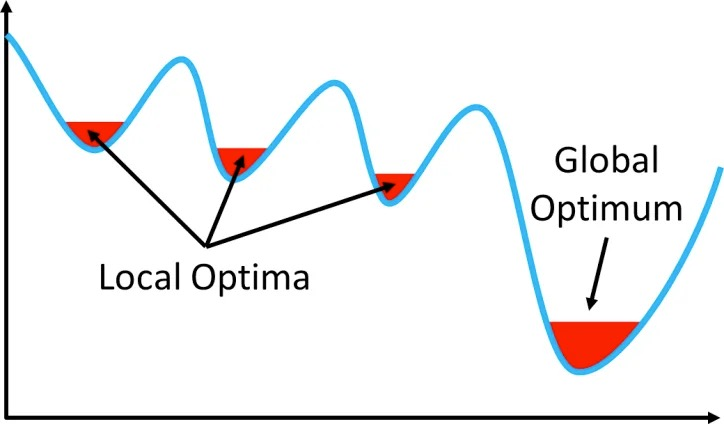
\includegraphics[width=0.22\textwidth]{Lec4/Local minimum and global minimum}
        \caption{Local minimum and global minimum}
    \end{figure}
    \begin{figure}[H]
        \centering
        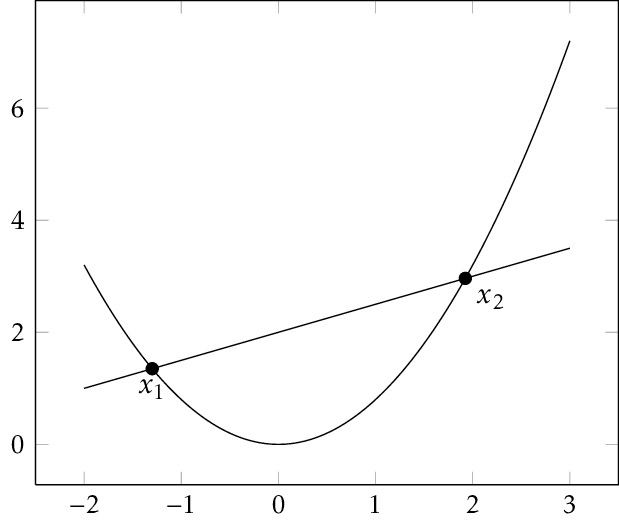
\includegraphics[width=0.22\textwidth]{Lec4/Convex optimization}
        \caption{Convex optimization}
    \end{figure}
    凸函数与凸优化是非常重要的(因为凸函数的局部最优就是全局最优), 把目标函数写成凸函数也有许多方法, 课外学习()

    \section{Robust estimation(鲁棒估计)}
    
    \subsection{Outliers(离群值)}
    \begin{itemize}
        \item Inlier: obeys the model assumption
        \item Outlier: differs significantly from the assumption
    \end{itemize}
    \begin{figure}[H]
        \centering
        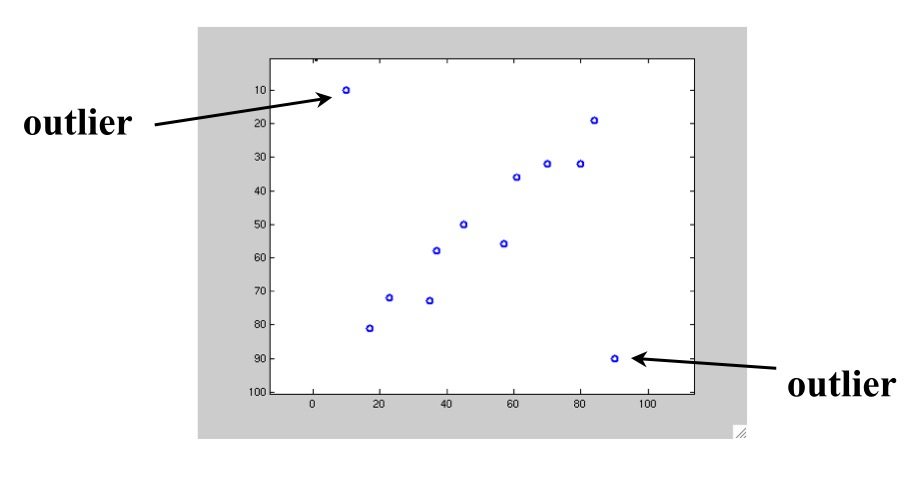
\includegraphics[width=0.22\textwidth]{Lec4/异常值}
        \caption{离群值}
    \end{figure}
    \subsection{Reduce the effect of Outliers}
    \begin{enumerate}
        \item Use other loss function to replace MSE, like L1, Huber. They are called robust functions.
        \begin{figure}[H]
            \centering
            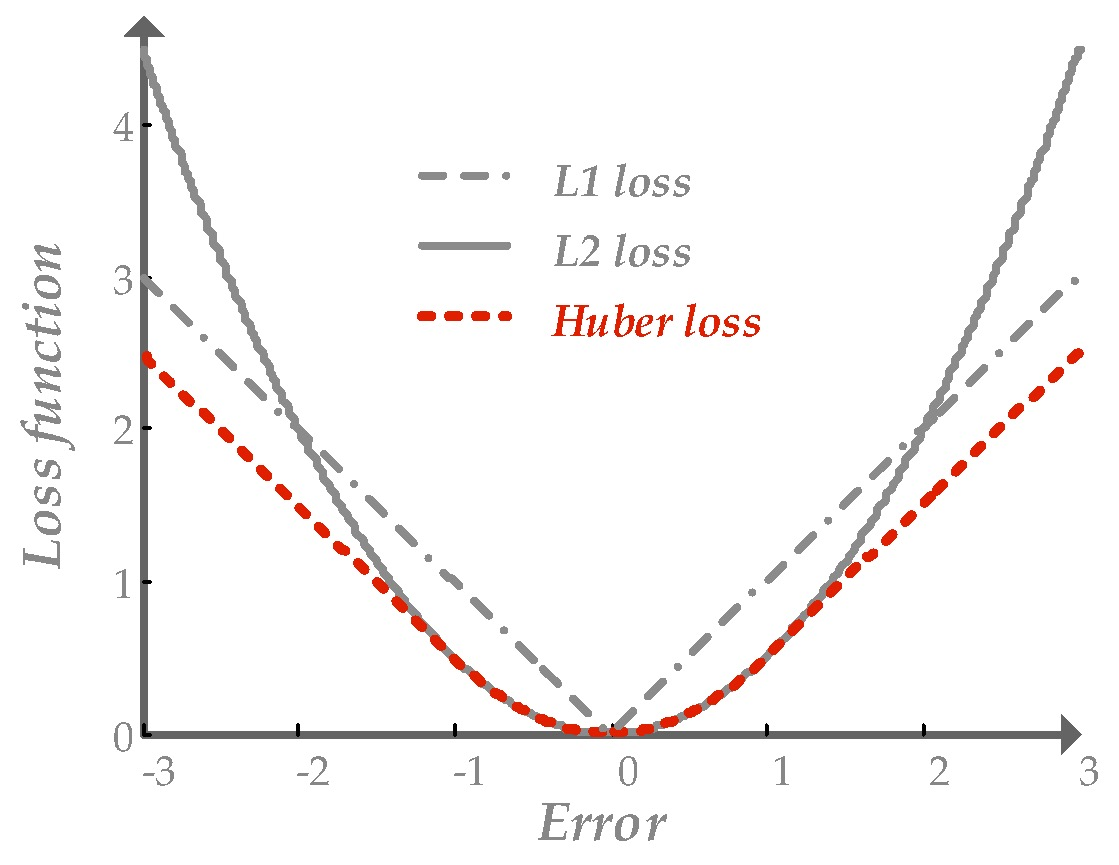
\includegraphics[width=0.22\textwidth]{Lec4/other loss functions}
            \caption{other loss function}
        \end{figure}
        \item RANSAC: Random Sample Concensus(随机一致采样)
        \begin{itemize}
            \item The most powerful method to handle outliers.
            \item Key ideas:
            \begin{itemize}
                \item The distribution of inliers is similar while outliers differ a lot.(好的数据的分布是近似的)
                \item  Use data point pairs to vote.(用点对连线进行投票积分, 求到最好的线后再用最小二乘跑一遍)
            \end{itemize}
        \end{itemize}
    \end{enumerate}
    \subsection{well-posed problem \& ill-posed problem(适定问题与病态问题)}
    Well-posed problem is 
    \begin{enumerate}
        \item a solution exists;
        \item  the solution is unique;
        \item the solution's behavior changes continuously with the initial conditions. (stable)
    \end{enumerate}

    当上面三者有一不满足时, 就是 ill-posed problem. 

    For the solution is not unique, eg: $Ax=b$ when A is singular matrix.

    How to make the soultion unique? Use prior knowledge to add more constraints(使用先验条件添加更多约束).
    \subsubsection{L2 regularization(正则)} 
    \begin{enumerate}
        \item L2 norm: $\left\| x \right\|_2=\sum_i x_i^2$
        \item L2 regularization:
        \begin{align*}
            \min_x &\left\| Ax-b \right\|_2^2\\
            s.t.&\left\| x \right\|_2\le 1
        \end{align*}

        \begin{figure}[H]
            \centering
            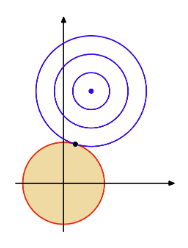
\includegraphics[width=0.22\textwidth]{Lec4/L2}
            \caption{L2}
        \end{figure}
        \begin{itemize}
            \item 把 x 往原点去拉. 
            \item 让参数趋近于零, 以此抑制没必要的小参数. 
        \end{itemize}
    \end{enumerate}

    \subsubsection{L1 regularization}
    \begin{enumerate}
        \item L1 norm: $\left\| x \right\|_1=\sum_i \left|x_i\right|$
        \item L1 regularization:
        \begin{align*}
            \min_x &\left\| Ax-b \right\|_2^2\\
            s.t.&\left\| x \right\|_1\le 1
        \end{align*}

        \begin{figure}[H]
            \centering
            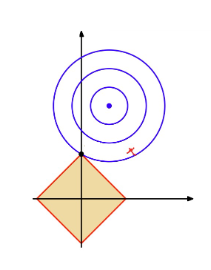
\includegraphics[width=0.22\textwidth]{Lec4/L1}
            \caption{L1}
        \end{figure}

        \begin{itemize}
            \item 有L2的优点.
            \item 让一些变量真的变为0(稀疏, sparse).
        \end{itemize}
    \end{enumerate}

    \subsection{Overfitting and underfitting(过拟合与欠拟合)}
    \begin{figure}[H]
        \centering
        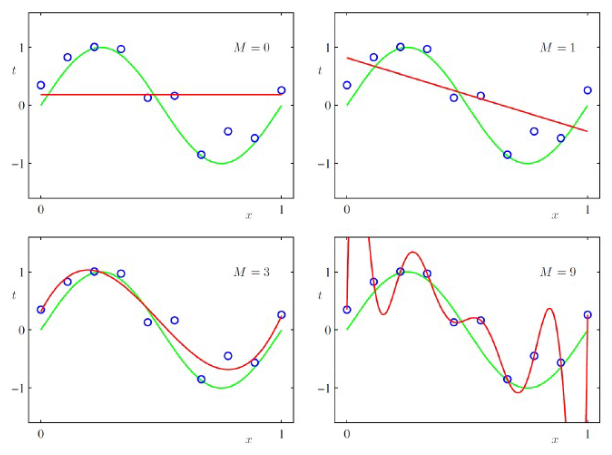
\includegraphics[width=0.38\textwidth]{Lec4/fitting}
        \caption{Overfitting and underfitting}
    \end{figure}

\section{Graphcut and MRF}
\subsection{Image labeling problems}
eg: Image segmentation(分割)

\subsubsection{Images as Graphs}
\begin{itemize}
    \item A vertex for each pixel
    \item An edge between each pair
    \item Graph Notation: G=(V, E)
    \item Each edge is weighted by the affinity or similarity between its two vertices(边权以像素相似性定义)
\end{itemize}
\subsubsection{Measuring affinity}
Let $i$ and $j$ be two pixels whose features are $f_i$ and $f_j$
\begin{itemize}
    \item Pixel Dissimilarity
    \begin{align*}
        S(f_i,f_j)=\sqrt{\sum_k(f_ik-f_jk)^2}
    \end{align*}
    \item Pixel Affinity(亲和性)
    \begin{align*}
        w(i,j)=A(f_i,f_j)=e^{-\frac{1}{2\sigma^2}S(f_i,f_j)}
    \end{align*}
\end{itemize}

\subsubsection{Graph cut}
Cut $C=(V_A, V_B)$ is a partition of vertices $V$ of a graph $G$ into two disjoint subsets $V_A$ and $V_B$.

Cost of Cut: Sum of weights of cut-set edges
\begin{align*}
    cut(V_A,V_B)=\sum_{u\in V_A, v\in V_B}w(u,v)
\end{align*}

让这个代价最小. 因为是离散的所以不能用上节课的优化方式. 

\paragraph{min-cut}
不过可以用最大流算法求最小割来解决. 

Problem:解不一定有意义(如把一个点视为一个子图).由此可见目标函数不够好. 
\begin{figure}[H]
    \centering
    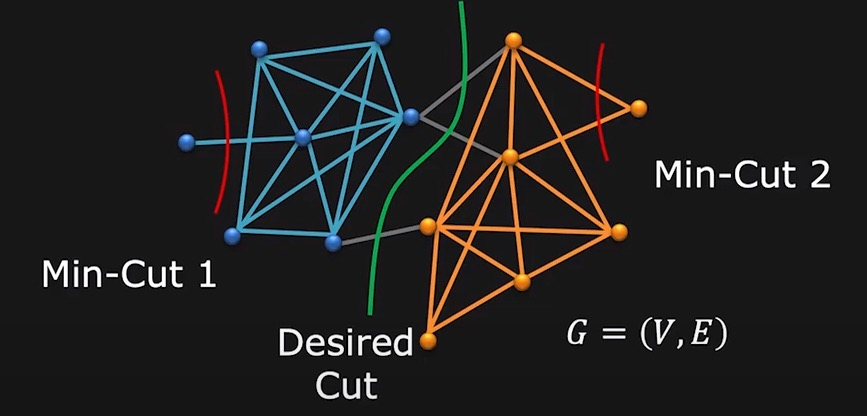
\includegraphics[width=0.38\textwidth]{Lec4/min-cut}
    \caption{min-cut}
\end{figure}

\paragraph{Normalized cut}
Normalizing for size of segments
\begin{align*}
    NCut(V_A,V_B)&=\frac{cut(V_A,V_B)}{assoc(V_A,V)}+\frac{cut(V_A,V_B)}{assoc(V_B,V)}\\
    assoc(V_a,V)&=\sum_{u\in V_A, v\in V} w(u,v)
\end{align*}
\begin{itemize}
    \item 为NP-Complete
    \item Approximate solution by eigenvalue
    decomposition.(但可以用特征值分解方法求近似解)
\end{itemize}

\subsection{Markov Random Field}
\subsubsection{Markov chains}
\begin{figure}[H]
    \centering
    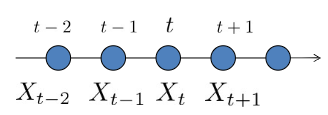
\includegraphics[width=0.38\textwidth]{Lec4/Markov chains}
    \caption{Markov chains}
\end{figure}
Markov chains用来描述一个系统随时间推移的状态转移。

在Markov chains中,系统在每个时刻都处于某一个状态,并且下一个状态只与当前状态有关,不受之前状态的影响。

\subsubsection{Markov Random Field}
\begin{figure}[H]
    \centering
    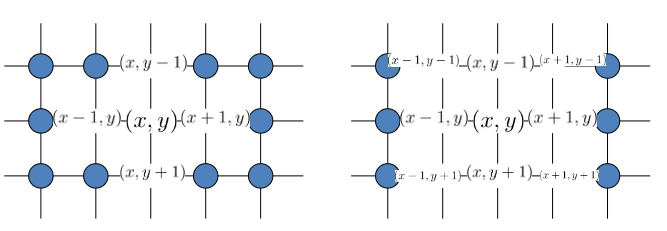
\includegraphics[width=0.38\textwidth]{Lec4/Markov random field}
    \caption{Markov random field}
\end{figure}
\begin{align*}
    P(I_{x,y}|I_{-(x,y)})=P(I_{x,y}|I_{N(x,y)})
\end{align*}

$-(x,y)$为其他所有点, $N(x,y)$为与之相邻的点.

每个像素的连续性只取决于与之相邻的像素. 即相邻变量之间有约束. 

\subsubsection{Segmentation by MRF}
Joint probability(联合概率分布)(此下x,y与上文x,y的意义并不相同)
\begin{figure}[H]
    \centering
    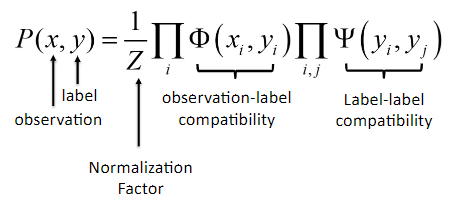
\includegraphics[width=0.38\textwidth]{Lec4/MRF}
    \caption{Segmentation by MRF}
\end{figure}
\begin{itemize}
    \item x为观测
    \item y为标签
    \item Z为常数
    \item $\prod_i\Phi(x_i,y_i)$所有像素的某个量相乘, 描述每个像素标签与观测的关系.
    \item $\prod_{i,j}\Psi (y_i,y_j)$相邻像素标签之间的关系.
\end{itemize}

需要最大化这个值, 等效于最小化其-ln, 即

Energy funciton
\begin{align*}
    E(x,y)=\sum_i \varphi(x_i,y_i)+\sum_{i,j}\psi(y_i,y_j)
\end{align*}

\begin{enumerate}
    \item Unary potentials(单一) $\varphi(x_i,y_i)$
    \begin{itemize}
        \item 每个像素自己标签的概率.
    \end{itemize}
    \item Pairwise potentials(成对) $\psi(y_i,y_j)$
    \begin{itemize}
        \item 成对像素标签中的一致性.
    \end{itemize}
\end{enumerate}

\subsubsection{Example}
\begin{enumerate}
    \item Unary potentials(单一) $\varphi(x_i,y_i)=(bool)(x_i \ne y_i)$
    \begin{itemize}
        \item 像素是否与标签一致, 不一致给 loss
    \end{itemize}
    \item Pairwise potentials(成对) $\psi(y_i,y_j)=(bool)(y_i = y_j)w_{ij}$
    \begin{itemize}
        \item 标签相同给 loss
    \end{itemize}
\end{enumerate}

How to solve?
\begin{itemize}
    \item 最大流求最小割Maxflow/Min-Cut
    \item 优化问题
\end{itemize}

\subsubsection{Advantage}
很好用, 用的很广泛. 

\subsubsection{Disadvantages}
多个标签只能近似求解. 